%!TEX root = ../../book_ML.tex
\section{Học chuyển tiếp cho bài toán phân loại ảnh}
% (\textit{Giả sử rằng bạn đọc đã có kiến thức nhất định về deep neural network.})
Mục này được viết trên cơ sở bạn đọc đã có kiến thức nhất định và deep learning.
% Trước khi deep learning ra đời, bài toán phân loại ảnh (các loại dữ liệu khác cũng tương tự) thường được chia thành hai bước: Feature Engineering và Train a Classifier. Hai bước này thường được tách rời nhau. 

Ngoài BoW, các phương pháp phổ biến được sử dụng để xây dựng vector đặc trưng cho ảnh là \textit{scale invariant feature transform -- SIFT}~\cite{lowe1999object}, \textit{speeded-up robust features -- SURF}~\cite{bay2006surf}, \textit{histogram of oriented gradients -- HOG}~\cite{dalal2005histograms}, \textit{local binary pattern -- LBP}~\cite{lowe1999object},... Các bộ phân loại thường được sử dụng là SVM đa lớp (Chương~\ref{cha:multisvm}), {hồi quy softmax} (Chương~\ref{cha:softmax}), mã hóa thưa và học từ điển~\cite{wright2009robust,vu2016histopathological,vu2016fast}, rừng ngẫu nhiên~\cite{liaw2002classification},... 



% Với Feature Engineering, các phương pháp thường được sử dụng cho ảnh là \href{http://docs.opencv.org/3.1.0/da/df5/tutorial_py_sift_intro.html}{SIFT} (Scale Invariant Feature Transform), \href{http://docs.opencv.org/3.0-beta/doc/py_tutorials/py_feature2d/py_surf_intro/py_surf_intro.html}{SURF} (Speeded-Up Robust Features), \href{http://www.learnopencv.com/histogram-of-oriented-gradients/}{HOG} (Histogram of Oriented Gradients), LBP (Local Binary Pattern), etc. Các Classifier thường được sử dụng là \href{http://machinelearningcoban.com/2017/04/28/multiclasssmv/}{multi-class SVM}, \href{http://machinelearningcoban.com/2017/02/17/softmax/}{Softmax Regression}, Discriminative Dictionary Learning, Random Forest, etc. 
\index{dac@đặc trưng thủ công -- hand-crafted feature} 
Các đặc trưng được tạo bởi các phương pháp nêu trên thường được gọi là các
\textit{đặc trưng thủ công} ({hand-crafted feature}) vì chúng chủ yếu dựa
trên các quan sát về đặc tính riêng của ảnh và được xây dựng chung cho mọi loại
dữ liệu ảnh. Các phương pháp này cho kết quả khá ấn tượng trong một số trường
hợp. Tuy nhiên, chúng vẫn còn nhiều hạn chế vì quá trình tìm ra các đặc trưng và
các bộ phân loại là riêng biệt. Hơn nữa, các bộ trích chọn này chỉ tìm ra các
\textit{đặc trưng mức thấp} ({low-level features}) của ảnh.

Những năm gần đây, deep learning phát triển cực nhanh dựa trên lượng dữ liệu
huấn luyện khổng lồ và khả năng tính toán ngày càng được cải tiến của các máy
tính. Kết quả cho bài toán phân loại ảnh ngày càng được nâng cao. Bộ cơ sở dữ
liệu thường được dùng nhất là ImageNet (\url{https://www.image-net.org}) với 1.2
triệu ảnh cho 1000 nhãn khác nhau. Rất nhiều mô hình deep learning đã giành
chiến thắng trong các cuộc thi \textit{ImageNet large scale visual recognition
challenge -- ILSVRC} (\url{https://goo.gl/1A8drd}):
AlexNet~\cite{krizhevsky2012imagenet}, ZFNet~\cite{zeiler2014visualizing},
GoogLeNet~\cite{szegedy2015going}, ResNet~\cite{he2016deep},
VGG~\cite{simonyan2014very}. Nhìn chung, các mô hình này là các \textit{mạng neuron đa tầng} (multi-layer neural network). Các tầng phía trước thường là các \textit{tầng tích chập} (convolutional layer). Tầng cuối cùng là một \textit{tầng nối kín} (fully connected layer) và thường là một bộ hồi quy
softmax (xem Hình~\ref{fig:transferlearning}). Vì vậy đầu ra của tầng gần cuối
cùng có thể được coi là vector đặc trưng và hồi quy softmax chính là bộ phân
loại được sử dụng\footnote{hồi quy softmax là một thuật toán phân loại, tên gọi \textit{hồi quy} của nó mang tính lịch sử.}.
 
Việc bộ trích chọn đặc trưng và bộ phân loại được huấn luyện cùng nhau thông qua
tối ưu hệ số trong mạng neuron sâu khiến các mô hình này đạt kết quả tốt. Tuy
nhiên, những mô hình này đều bao gồm rất nhiều tầng các trọng số. Việc huấn
luyện dựa trên hơn một triệu bức ảnh tốn rất nhiều thời gian (2-3 tuần).
 
\index{học chuyển tiếp -- transfer learning}
Với các bài toán phân loại các dữ liệu ảnh khác với tập huấn luyện nhỏ, ta có
thể không cần xây dựng lại mạng neuron và huấn luyện nó từ đầu. Thay vào đó, ta có
thể sử dụng các mô hình đã được huấn luyện nêu trên và thay đổi kiến trúc của mạng cho phù hợp. Phương pháp sử dụng các mô hình có sẵn như vậy còn
được gọi là \textit{học chuyển tiếp} ({transfer learning}).
 
Toàn bộ các tầng trừ tầng đầu ra có thể được coi là một bộ trích chọn đặc trưng.
Điều này được rút ra dựa trên nhận xét rằng các bức ảnh thường có những đặc tính
giống nhau. Sau đó, ta huấn luyện một bộ phân loại khác dựa trên
vector đặc trưng đã đã được trích chọn. Cách làm này có thể tăng độ chính xác
phân loại lên đáng kể so với việc sử dụng các đặc trưng thủ công vì các mạng neuron sâu được cho là có khả năng trích chọn các \textit{đặc trưng mức cao} ({high-level features}) của ảnh. 

 
%% *****************************************************************************
\begin{figure}[t]
\centering
    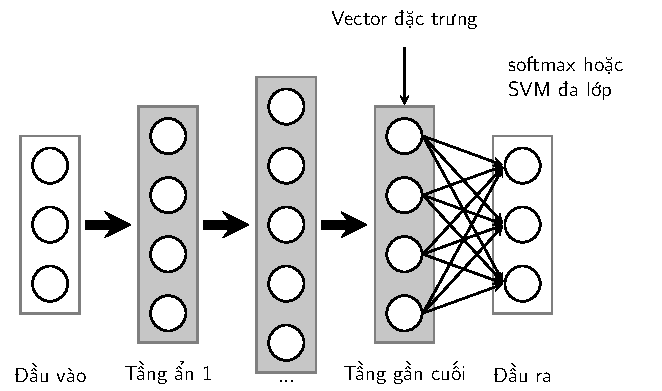
\includegraphics[width = \textwidth]{Chapters/01_Overview/q2_tl/latex/multi_layers.pdf}
    \caption[]{Kiến trúc deep learning cơ bản cho bài toán phân loại. Tầng cuối cùng là một tầng nối kín và thường là một hồi quy softmax.}
    \label{fig:transferlearning}
\end{figure}
%% ***************************************************************************** 
\index{tinh chỉnh -- fine-tuning}
Hướng tiếp cận thứ hai là sử dụng các mô hình đã được huấn luyện và cho huấn luyện thêm một vài tầng cuối dựa trên dữ liệu mới. Kỹ thuật này được
gọi là \textit{tinh chỉnh} ({fine-tuning}). {Việc này được thực hiện dựa trên quan
sát rằng những tầng đầu trong mạng neuron sâu trích xuất những đặc trưng chung mức thấp của đa số ảnh, các tầng cuối giúp trích chọn các đặc trưng mức cao phù hợp cho từng cơ sở dữ liệu (CSDL). Các đặc trưng mức cao có thể khác nhau tuỳ theo từng CSDL. Vì vậy, khi có dữ liệu mới, ta chỉ cần huấn luyện mạng neuron để trích chọn các đặc trưng mức cao phù hợp với dữ liệu mới này. 
 
Dựa trên kích thước và sự giống nhau giữa CSDL mới và CSDL gốc (dùng để huấn luyện mạng neuron ban đầu), có một vài quy tắc để huấn luyện mạng neuron mới\footnote{\textit{Transfer Learning, CS231n} (\url{https://goo.gl/VN1g7F})}: 

\begin{itemize}
\item \textit{CSDL mới nhỏ, tương tự CSDL gốc.} Vì CSDL mới nhỏ, việc
tiếp tục huấn luyện mô hình có thể dễ dẫn đến hiện tượng \textit{quá khớp} (overfitting, xem Chương~\ref{cha:overfitting}). Cũng vì hai CSDL tương tự nhau, ta dự đoán
rằng các đặc trưng mức cao của chúng tương tự nhau. Vì vậy, ta không cần
huấn luyện lại mạng neuron mà chỉ cần huấn luyện một bộ phân loại dựa trên các vector đặc trưng thu được. 
 
\item \textit{CSDL mới lớn, tương tự CSDL gốc.} Vì CSDL này lớn,
quá khớp ít xảy ra hơn, ta có thể huấn luyện mô hình thêm một
vài vòng lặp. Việc huấn luyện có thể được thực hiện trên toàn bộ hoặc chỉ một
vài tầng cuối.
 
\item \textit{CSDL mới nhỏ, rất khác CSDL gốc.} Vì CSDL này nhỏ, tốt
hơn hết là dùng các bộ phân loại đơn giản khác để tránh quá khớp. Nếu muốn sử
dụng mạng neuron cũ, ta cũng chỉ nên tinh chỉnh các tầng cuối của nó. Hoặc có thể coi đầu ra của một tầng ở giữa của mạng neuron là vector đặc
trưng rồi huấn luyện thêm một bộ phân loại.
 
\item \textit{CSDL mới lớn rất khác CSDL gốc.} Thực tế cho thấy, sử dụng
các mạng neuron sẵn có trên CSDL mới vẫn hữu ích. Trong trường hợp này, ta vẫn có
thể sử dụng các mạng neuron sẵn có như là điểm khởi tạo của mạng neuron mới, không nên
huấn luyện mạng neuron mới từ đầu.
\end{itemize}
 
Một điểm đáng chú ý là khi tiếp tục huấn luyện các mạng neuron này, ta chỉ
nên chọn tốc độ học nhỏ để các hệ số mới không đi quá xa so với các
hệ số đã được huấn luyện ở các mô hình trước.
 
 
 
 
 
% \section{Đọc thêm}
% [1] \href{http://docs.opencv.org/3.1.0/da/df5/tutorial_py_sift_intro.html}{Introduction to SIFT (Scale-Invariant Feature Transform) - OpenCV} 
 
% [2] \href{http://machinelearningcoban.comIntroduction to SURF (Speeded-Up Robust Features}{Introduction to SURF (Speeded-Up Robust Features) - OpenCV}) 
 
% [3] \href{http://www.learnopencv.com/histogram-of-oriented-gradients/}{Histogram of Oriented Gradients - OpenCV} 
 
% [4] \href{http://cs231n.github.io/transfer-learning/#tf}{Transfer Learning} 
 
% [5] \href{http://sebastianruder.com/transfer-learning/}{Transfer Learning - Machine Learning's Next Frontier} 
 
% [6] \href{https://www.analyticsvidhya.com/blog/2017/06/transfer-learning-the-art-of-fine-tuning-a-pre-trained-model/}{Transfer learning & The art of using Pre-trained Models in Deep Learning} 
